\section{Wstep teoretyczny} \label{theory}
W kolejnych podrozdziałach opisane są krótko podstawy teoretyczne dotyczące uczenia maszynowego, wykorzystanych algorytmów oraz użytych metod optymalizacji.
\subsection{Formalny opis uczenia maszynowego}
Uczenie maszynowe okreslane jest jako jedna z galezi sztucznej inteligencji \cite{dnn1}. Formalną definicję podał Tom Mitchell, która brzmi następująco: ,,Mówimy, że maszyna uczy się zadania $T$ w oparciu o doświadczenie $E$ i miarę jakości $P$, jeśli wraz z przyrostem doświadczenia $E$ poprawia się jakość wykonywanego zadania $T$ mierzona przez miarę $P$.''\cite{mitchel} Przykładowo można wymienić trójkę $T$, $E$, $P$ jako diagnozowanie pacjenta na podstawie symptomów, dotychczasowe  liczba wykonanych przez maszynę diagnoz (poprawnie lub nie),  poprawność diagnozowania na podstawie do tej pory niespotkanych przypadków. Powyższe przykłady można mnożyć. Zapis formalny (na podstawie \cite{formal2}) w przypadku algorytmów przedstawionych w nieniejszej pracy możemy przedstawić następująco:
\begin{itemize}
\item $x$ - dane wejściowe algorytmu
\item $y$ - wyjście algorytmu
\item $f$ - funkcja modelowana
\item $g$ - funkcja modelująca.
\end{itemize}
Ogólnie możemy powiedzieć, że zadaniem algorytmu jest znalezienie takiej funkcji $g$, która jak w najlepszy stopniu przybliża funkcję $f$. Odnosząc to do przykładu rozpoznawania chorób, możemy powiedzieć, że modelowaną funkcją jest funkcja symptomów, która przyporządkowuje pacjentowi diagnozę. Uczenie wg danego algorytmu przeprowadza się na podstawie danych:
\begin{equation}
d = (x_1,y_1), (x_2, y_2), ..., (x_n, y_n).
\end{equation}
Każda para $(x_i, y_i)$ stanowi jeden rekord danych lub też jeden przykład podawany do algorytmu. W odniesieniu do przykładu z rozpoznawaniem chorób na podstawie symptomów, jednym rekordem jest konkretny zestaw symptomów ($x_i$) wraz z diagnozą ($y$).  Ogólniej, poszczególne symptomy nazywa się cechami lub atrybutami. W zależności od tego czy $y$ przyjmuje wartości ciągłe czy dyskretne, mamy do czynienia z wykorzystaniem uczenia maszynowego w problemie kolejno regresji lub klasyfikacji. W kolejnych podrozdziałach autor korzysta również z określenia niestabilny algorytm uczenia maszynowego. Mamy z takim do czynienia, gdy mała zmiana w danych wejściowych może spowodować dużą zmianę w predykcjach generowanych przez algorytm\cite{ensamble}.
%W tej pracy wszystkie metody optymalizacji były analizowane pod kątem problemu klasyfikacji lecz naturalne jest ich użycie w przypadku problemu regresji.

\subsection{Wykorzystane algorytmy}
W tym podrozdziale opisane są kolejne algorytmy, które wykorzystywane były w pracy.
\subsubsection{Drzewo decyzyjne}
%www.cs.princeton.edu/courses/archive/spr07/cos424/papers/mitchell-dectrees.pdf
% scikit-learn uses an optimised version of the CART algorithm.
Drzewo decyzyjne jest algorytmem uczenia maszynowego, który może posłużyć w celu rozwiązania problemu klasyfikacji oraz regresji. Funkcja, która jest modelowana przez algorytm przedstawiana jest w formie drzewa matematycznego. Jest to jedna z najpopularniejszych metod, która znalazła swoje wykorzystanie w diagnozowaniu chorób czy ocenie ryzyka kredytowego klientów banków\cite{mitchel}. Zaletami tego podejścia jest między innymi  prostota oraz łatwość interpretacji. Dużą wadą drzew decyzyjnych jest fakt, iż stworzenia optymalnego drzewa decyzyjnego należy do klasy problemów NP-zupełnych. W praktyce tworzenie drzewa oparte jest na metodach heurystycznych\cite{dtscikit}. Na rysunku \ref{dt1image} przedstawione zostało przykładowe drzewo, które mogłoby posłuży do klasyfikacji danych o trzech atrybutach na trzy klasy. Można stwierdzić, że drzewo decyzyjne jest tzw. białą skrzynką (\textit{whitebox}), ponieważ łatwo można zauważyć na jakiej podstawie podjęta została decyzja przyporządkowania do danej klasy.

\begin{figure}[ht!]
\centering
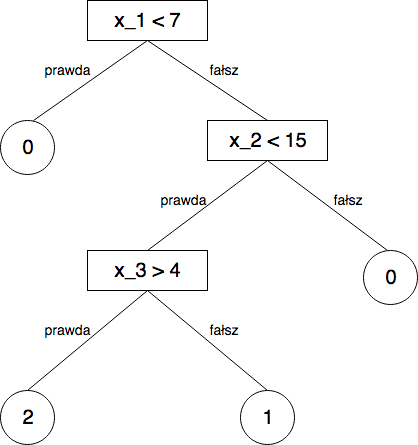
\includegraphics[scale=0.6]{res/dt1.png}
\caption[Caption for LOF]{Przykład drzewa decyzyjnego.\label{dt1image}}
% \caption{Matematyczny model neuronu\label{neuron} Źródło:\footnote{aa} } 
\end{figure} 

\paragraph{Tworzenie drzewa decyzyjnego}\mbox{}\\
%ftp://ftp.boulder.ibm.com/software/analytics/spss/support/Stats/Docs/Statistics/Algorithms/14.0/TREE-CART.pdf
Istnieją różne sposoby na stworzenie drzewa klasyfikacyjnego. Jednym z nich jest algorytm CART -\textit{Classification  and  Regression  Trees}, który był wykorzystany w tej pracy i jest opisany w tym paragrafie. Ideą tego podejścia jest dzielenie danych wejściowych na rozłączne i dopełniające się podzbiory w taki sposób, aby zbiory te pozostawały jak najbardziej jednorodne tj. posiadały jak najwięcej rekordów przynależących do tej samej kategorii. Budowa drzewa zaczyna się od jego korzenia. Wybieramy atrybut wg którego chcemy podzielić dane na dwa jak najbardziej jednorodne zbiory. Po podzieleniu zbioru na dwa podzbioru postępujemy tak samo z następnymi atrybutami. Podział przeprowadzany jest aż do momentu, gdy wszystkie rekordy w każdym podzbiorze przynależą do tej samej kategorii. Należy jednak określić wg których atrybutów dzielić dane tak aby powstawały jak najbardziej jednorodne zbiory. W tym celu wykorzystywane są różnego rodzaju kryteria jednorodności\cite{CART}. Cały algorytm, w uproszczeniu, można opisać w dwóch krokach:
\begin{enumerate}
\item Wybór atrybutu, który pozwoli podzielić zbiór na dwa najbardziej jednorodne podzbiory.
\item Podział wg atrybutu wybranego w kroku 1 jeżeli nie zostały spełnione warunki końca algorytmu\cite{CART}.
\end{enumerate}
Warunkiem końca algorytmu może być sytuacja w której wszystkie stworzone podzbiory są jednorodne lub też moment, gdy dotarliśmy do maksymalnej głębokości drzewa. Każdy podzbiór oznacza kolejną gałąź w drzewie, co powoduje wzrost drzewa. Gdy drzewo jest zbyt duże, staję się ono zbyt skomplikowane i podatne na przeuczenie(\textit{overfitting}). Jednym z parametrów drzewa decyzyjnego, który należy określić jest właśnie jego maksymalna głębokość, która pozwala stworzyć optymalne drzewo. Wspomniany problem przeuczenia został opisany w podrozdziale \ref{problems}. 

\subsubsection{Las drzew decyzyjnych}
%http://jair.org/media/614/live-614-1812-jair.pdf
Las drzew decyzyjnych(\textit{Random forest}) powstał na podstawie idei tworzenia silnego klasyfikatora na podstawie $n$ słabych klasyfikatorów tego samego typu. Podejście to w literaturze określane jest jako \textit{ensable learning}. Szczególnym przypadkiem tego podejścia jest tzw. \textit{bagging}\cite{gonczarek}. Koncepcję \textit{ensable learning} można zobrazować przedstawiając wiele wielomianów, które nie modelują zbyt dobrze funkcji $f$, lecz ich uśrednianie już realizuje to znacznie lepiej, co zostało przedstawione na rysunku \ref{avg1}.  W przypadku uczenia klasyfikatora typu \textit{bagging} tworzymy $m$ klasyfikatorów, każdy z nich uczymy używając $N$ rekordów, który losujemy z powtórzeniami korzystając ze zbioru danych o rozmiarze $N$. Implikuje to fakt, że niektóre ze słabych klasyfikatorów uczone będą na przykładach, które się powtarzają lub niektóre z przykładów w ogóle nie zostaną wzięte pod uwagę. Poszczególne klasyfikatory z pewnością będą cechowały się mniejszą skutecznością jeśli chodzi o klasyfikację, ale ich uśredniony wynik zazwyczaj daje lepsze rezultaty. Wykorzystanie sprawdza się najczęściej w przypadku niestabilnych algorytmów uczenia maszynowego do których zaliczyć też można drzewa decyzyjne\cite{ensable}. Duża zaletą algorytmów typu \textit{bagging} jest fakt, iż ich zrównoleglanie jest bardzo naturalne.
W przypadku lasu drzew decyzyjnych, jak nazwa wskazuje, mamy do czynienia z zespołem słabych klasyfikatorów, które są drzewami decyzyjnymi. Dodatkowo, w celu uczenia poszczególnych drzew, wykorzystujemy tylko $M$ atrybutów zbioru uczącego. Przy czym zaleca się, aby $M=\sqrt{K}$, zakładając, że $K$ oznacza liczbę wszystkich atrybutów zbioru uczącego. Podstawowymi parametrami lasu drzew decyzyjnych, które należy wyznaczyć jest liczba słabych klasyfikatorów wchodzących w skład klasyfikatora oraz maksymalna głębokość wykorzystanych drzew decyzyjnych.
\begin{figure}[ht!]
\centering
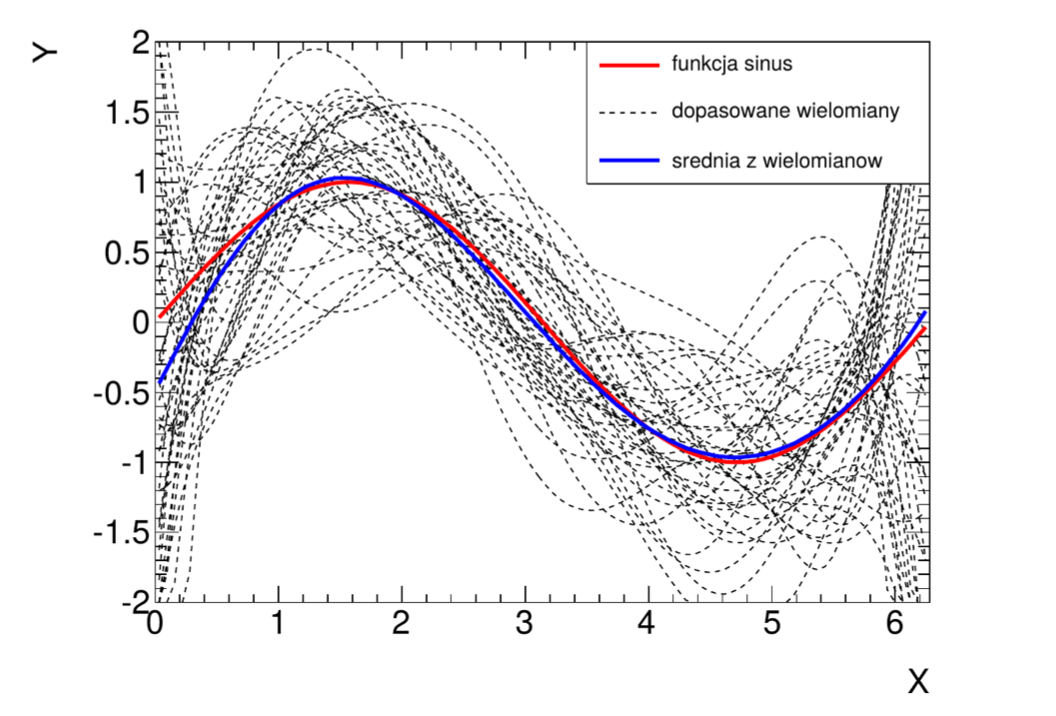
\includegraphics[scale=0.7]{res/avg1.png}
\caption[Caption for LOF]{Ilistracja działania \textit{ensamble learning} TODO:Podać źródło?\label{avg1}}
\end{figure} 

\subsubsection{Maszyna wektorow nosnych}
Maszyna wektorów wspierających (\textit{support vector machine - SVM}) jest modelem matematycznym, który z powodzeniem znajduje swoje zastosowaniu w klasyfikacji oraz regresji. Jej idea jest z jednej strony dość prosta, natomiast z drugiej sprawdza się w dość skomplikowanych problemach\cite{svm1}. Na rysunku \ref{svmIdea} przedstawiona został pomysł, który kryje się za tym algorytmem. Celem jego działania jest znalezienie hiperpłaszczyzny, która dzieli dane wg klas w optymalny sposób. W tym celu, wybierana jest hiperpłaszczyzna, która dzieli dane na dwie klasy zachowując przy tym jak największą odległość od punktów obu tych klas\cite{svm2}. Podstawowa wersja tego algorytmu zapewnia tylko klasyfikacje binarną tzn. taką w przypadku której mamy tylko dwie klasy. W celu rozszerzenia jego działania, istnieją dwa popularne podejścia  tj. \textit{one against one} oraz \textit{one against all}\cite{svm3}. W niniejszej pracy wykorzystane zostało pierwsze z nich, które polega na stworzeniu maszyny wektorów wspierających dla każdej pary klas. Wynika z tego, że konieczne jest stworzenie $K(K-1)/2$ maszyn, zakładając, że $K$ oznacza liczbę atrybutów analizowanego zbioru danych. Ostatecznie, klasa dla konkretnego rekordu danych określana jest poprzez ,,głosowanie''. Ostatnią podstawową kwestią, którą należałoby wyjaśnić, jest pytanie jak \textit{SVM} radzi sobie w przypadku, gdy dane nie są separowalne liniowo, przy których jest również wielokrotnie wykorzystywana. W takiej sytuacji wykorzystana jest transformacja danych, które pozwala na przedstawienie je w przestrzeni w której są one separowalne liniowo. Zobrazowanie tego rozwiązania przedstawia rysunek \ref{svmKernel}. Algorytm dąży do maksymalizacji odległości marginesu, który powstaje podczas dobierania hiperpłaszczyzny (patrz rys \ref{svmIdea}. W wielu przypadkach nie jest możliwe dobranie takiej hiperpłaszczyzny, która dokładnie podzieli dane. Rozwiązaniem w tej sytuacji jest dodanie dodatkowego współczynnika $C$, który dodatkowo uwzględniany jest w procesie optymalizacji. Wartość $C$ stanowi o tym jak duży wpływ na optymalizację mają niepoprawnie sklasyfikowane przykłady w procesie maksymalizacji marginesu i jest jednym z parametrów modelu, który należy wyznaczyć w celu otrzymania najbardziej optymalnego klasyfikatora.

\begin{figure}[ht!]
\centering
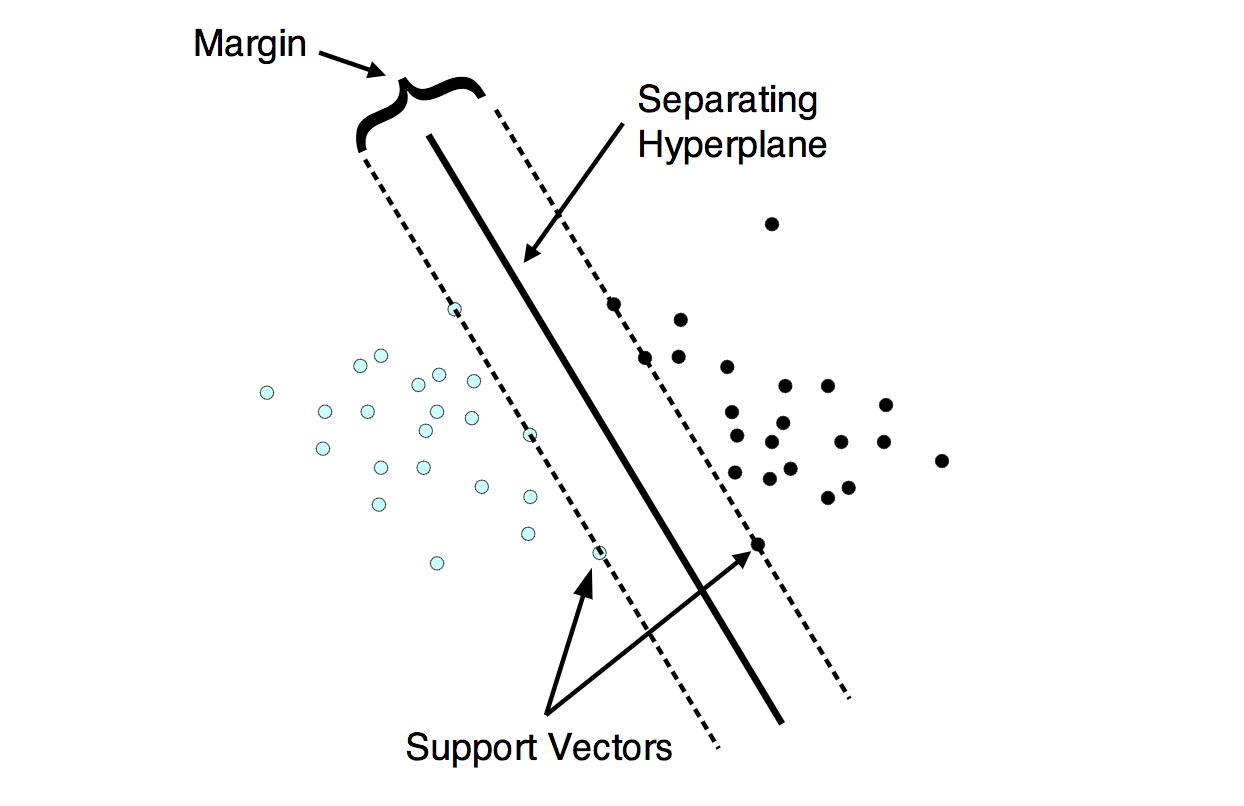
\includegraphics[scale=0.8]{res/svm1.png}
\caption[Caption for LOF]{Rysunek przedstawiający ideę maszyny wektorów wspierających. Źródło:\cite{svm2} \label{svmIdea}}
\end{figure} 

\begin{figure}[ht!]
\centering
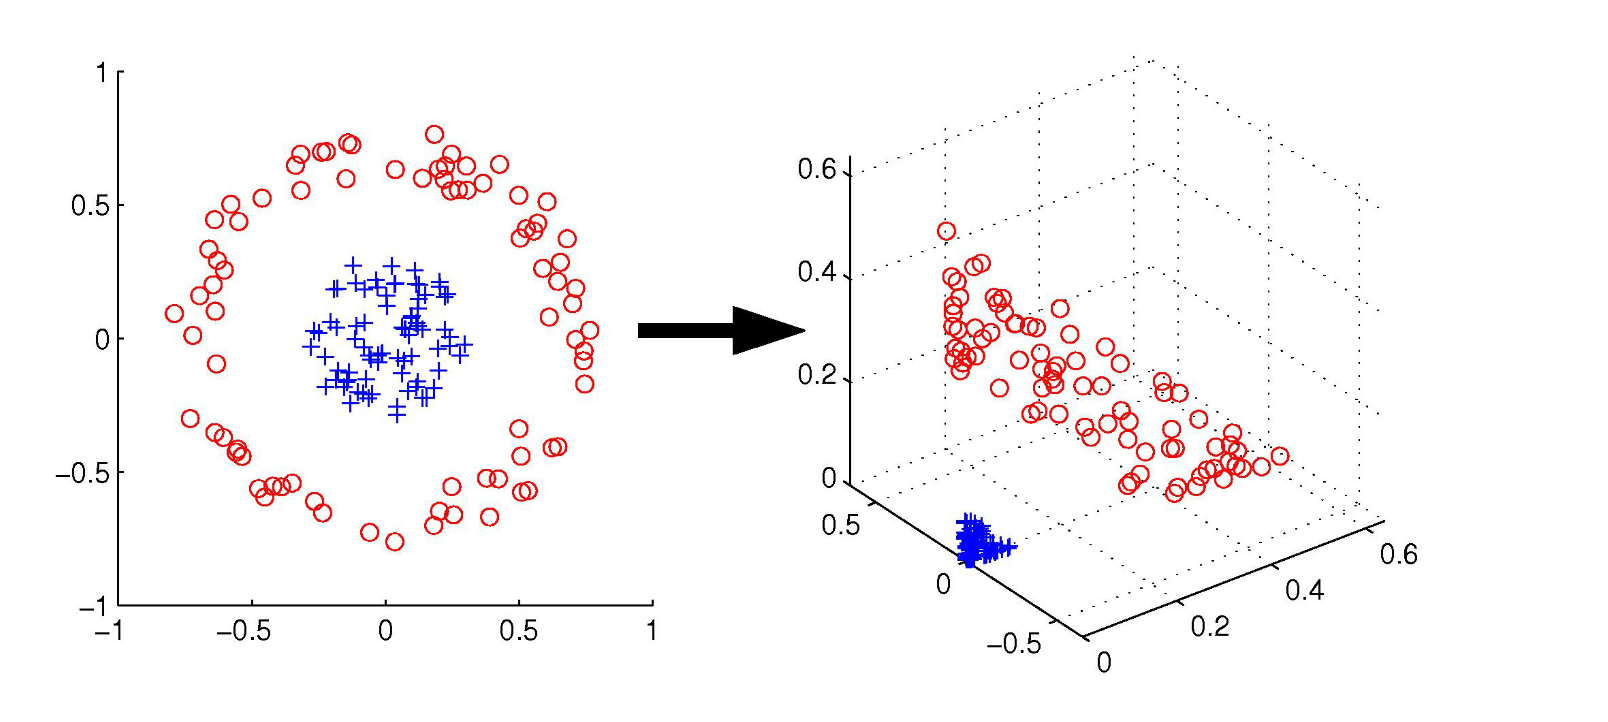
\includegraphics[scale=0.6]{res/svm2.png}
\caption[Caption for LOF]{Rysunek przedstawiający ideę transformowania danych do przestrzeni w której są one liniowo separowalne. Źródło:\cite{svmKernel} \label{svmKernel}}
\end{figure} 

\subsubsection{Tradycyjne sieci neuronowe}
% sieci neuronowe jako blackbox?
Niniejszy podrozdział powstał na podstawie pracy \cite{tadeusiewicz}. Sztuczna sieć neuronowa, dalej nazywana siecią neuronową, jest metodę uczenia maszynowego, którego inspiracją była biologia, a konkretnie ludzki mózg i występujące w nim biologiczne sieci neuronowe. Podstawową odmianą sieci neuronowej jest sieć jednokierunkowa, czyli taka w której nie występują sprzężenia zwrotne. Podstawową jednostką budulcową tego modelu jest neuron, który przedstawiony został na rysunku \label{neuron}. Pojedynczy neuronu wykonuje operację sumy ważonej korzystając z wartości na swoich wejściach oraz wagi przypisanej do każdego wejścia. Wyjście z kolei jest wynikiem zastosowania tzw. funkcji aktywacji na wyniku uprzednio otrzymanym z operacji sumy ważonej. Najpopularniejszymi funkcjami aktywacji w tradycyjnych sieciach neuronowych są funkcja sigmoidalna oraz  tangensoidalna. TODO: I jeszcze moze ta relu?
 
\begin{figure}[ht!]
\centering
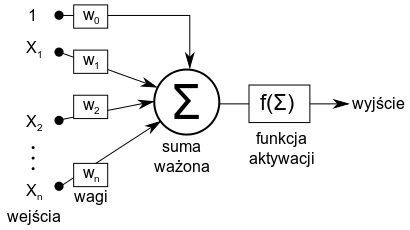
\includegraphics{res/neuron.png}
\caption[Caption for LOF]{TODO:footnotetext on wrong page Matematyczny model neuronu\label{neuron}\footnotemark}
% \caption{Matematyczny model neuronu\label{neuron} Źródło:\footnote{aa} } 
\end{figure} 
\footnotetext{\url{http://pl.wikipedia.org/wiki/Plik:
Neuron_McCullocha-Pittsa.png}}


Cała sieć neuronowa jest niczym innym niż połączonymi ze sobą neuronami. Każdemu połączeniu przypisana jest waga liczbowa, która informuje o tym jak wpływają na siebie poszczególne komórki sieci. Wszystkie neurony zgrupowaną są w warstwy z których możemy wyróżnić:
\begin{itemize}
\item warstwę wejściową
\item jedną lub więcej warstw ukrytych
\item warstwę wyjściową
\end{itemize}

W każdej warstwie może znajdować się dowolna ilość neuronów. Przykład sieci neuronowej został przedstawiony na rysunku \label{net}.

\begin{figure}[ht!]
\centering
% obrazek pobrany z 
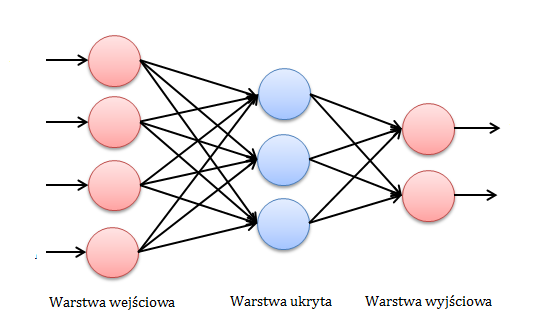
\includegraphics{res/exampleNet.png}
\caption[Caption for LOF]{Przykładowa jednokierunkowa sieć neuronowa\label{net}\footnotemark} 
\end{figure}

\footnotetext{\url{https://2ml4pa.bn1303.livefilestore.com/y2p6no6Dn0weHW3FG9tceTUS9lohx5ldcxvFZRhKdbeFQi2kntad_77gKeKIC-INcsFRCvGI-_DY9lMdZzaX8jkSHDvqlcT3qRnftpAt7esi4s/1.PNG?psid=1}}

W każdej iteracji uczenia sieci, na wejście podawany są dane. W zależności o odpowiedzi otrzymanej przez sieć przeprowadzana jest poprawa wag. Po przeprowadzeniu uczenia, sieć powinna ustalić wagi takie, aby poprawnie odpowiadać na kolejne sygnały wejściowe. W ogólności mówimy o minimalizacji błędu sieci $Q$ w zależności od wag sieci. W równaniu aktualizującym wagi występuję również współczynnik $\eta$, który jest tzw. współczynnikiem uczenia, który zmniejsza wprowadzane poprawy wag sieci. Dzięki temu współczynnikowi proces uczenia przebiega bardziej optymalnie. Jest on jednym z parametrów modelu, który należy wyznaczyć. Kolejnym z parametrów tego modelu jest liczba neuronów w warstwie ukrytej. Liczba neuronów w warstwie wejściowej zależy od liczby atrybutów naszych danych, natomiast wyjściowej od tego na ile kategorii dane są klasyfikowane. Pierwsze algorytmy uczenia, które powstały potrafiły przeprowadzić uczenie sieci neuronowej tylko o jednej warstwie. W celu uczenia sieci wielowarstwowych powstał algorytm wstecznej propagacji. Błąd dla poszczególnych neuronów jest w tym algorytmie obliczany ,,od przodu'' to znaczy zaczynając od warstwy wyjściowej. Dla neuronów w warstwie ukrytej błąd obliczany jako średnia ważona błędów neuronów do których dany neuron wysłał swój sygnał.
\subsubsection{Głębokie sieci neuronowe}
Niniejszy rozdzial zostal napisany na podstawie\cite{dnn1}.\\
% https://stats.stackexchange.com/questions/182734/what-is-the-difference-between-a-neural-network-and-a-deep-neural-network
% https://arxiv.org/pdf/1703.09039.pdf
Ideą stojącą za głębokimi sieciami neuronowymi jest tworzenie sieci, które posiadają wiele warstw ukrytych. Wiele, to znaczy od kilku do nawet kilku tysięcy. W tradycyjnych sieciach neuronowych zazwyczaj występowało co najwyżej kilka warstw ukrytych, a bardzo często tylko jedna. Udowodnione zostało matematycznie, że sieć o takiej strukturze jest zdolna do modelowania jakiejkolwiek funkcji pod warunkiem występowania w niej nieliniowych funkcji aktywacji w neuronach. W przypadku tradycyjnych sieci neuronowych na wejście sieci podawane są atrybuty, które należy samemu określić. Są to wyznaczone matematycznie cechy w zależności od problemu. Przykładem takiej sytuacji możesz być rozpoznawanie konkretnych obiektów na obrazie. Do sieci neuronowej możemy podać w takiej sytuacji konkretnie wyliczone cechy obrazu zamiast przekazywać wartość każdego piksela, co powodowałoby, że sieć miałaby bardzo dużo wejść, a co za tym idzie, trudno byłoby ją nauczyć. Takimi cechami mogą być np. jasność obrazu, tekstura, wskaźnik występujących na obrazie linii lub okręgów oraz wiele więcej. Przy operacji ekstrakcji cech z obrazu następuję naturalnie pewna utrata informacji. W przypadku głębokich sieci neuronowych nie dokonujemy ekstrakcji cech co jest zasadniczą różnicą. Na wejście sieci podawany są dane w stanie ,,surowym''. Pozwala to na uniknięcie utraty informacji co przy odpowiedniej ilości danych oraz dobrze zbudowanej sieci pozwala na znacznie lepsze wyniki. Sieć podczas procesu uczenia jest w stanie sama nauczyć się jakie cechy powinna rozpoznawać. Różnica ta została zilustrowana na rysunku \ref{dnnDiff}.

\begin{figure}[ht!]
\centering
% obrazek pobrany z 
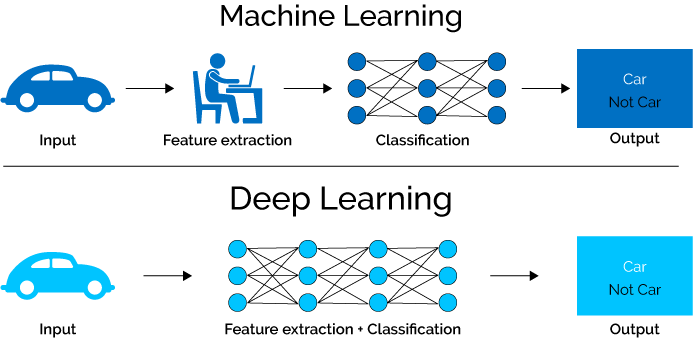
\includegraphics[scale=0.5]{res/dnn1.png}
\caption[Caption for LOF]{Różnica tradycyjnych sieci neuronowych oraz głębokich sieci neuronowych w kontekście ekstrakcji cech\label{dnnDiff}\footnotemark} 
\end{figure}
\footnotetext{\url{https://hackernoon.com/log-analytics-with-deep-learning-and-machine-learning-20a1891ff70e}}

\subsubsection{Konwolucyjne sieci neuronowe}
Niniejszy rozdział został napisany na podstawie\cite{nielsen}.\\
Konwolucyjne sieci neuronowe są najpopularniejszym typem głębokich sieci neuronowych. Znajdują swoje zastosowanie wszędzie, gdzie możemy zetknąć się z potrzebą analizy obrazów. Ich nazwa wynika wynika z faktu, iż bazują one na operacji konwolucji. W przypadku tradycyjnych sieci neuronowych, w sytuacji analizy obrazu bez ówczesnej ekstrakcji cech, należałoby podać na każde wejście sieci wartość pojedynczego piksela. Problemem tego podejścia jest to, że nie jest brana pod uwagę przestrzenna natura obrazu. Każde wejście sieci traktowane jest indywidualnie i nie jest ważne jego położenie na obrazie.  Konwolucyjne sieci neuronowe wykorzystują przestrzenną naturę obrazu. Ich architektura jest do tego dostosowana. Głównymi elementem sieci tego typu odróżniającymi je od tradycyjnych jest istnienie warstw konwolucyjnej. W przypadku tradycyjnych sieci neuronowych, zazwyczaj wyobrażamy sobie warstwę jako pojedyncza linie neuronów. Dla warstwy konwolucyjnej, bardziej naturalne jest jej przedstawienie w dwóch wymiarach.
\begin{figure}[ht!]
\centering
% obrazek pobrany z 
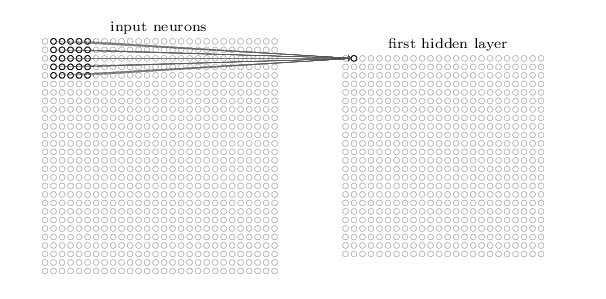
\includegraphics[scale=0.6]{res/cnn1.png}
\caption[Caption for LOF]{Warstwa wejściowa konwolucyjnej sieci neuronowej przedstawiona w dwóch wymiarach. Źródło:\cite{nielsen}\label{cnn1}} 
\end{figure}

Wartością każdego neuronu wejściowego jest wynik operacji konwolucji. W celu otrzymania wszystkich wejść należy ,,przesuwać'' maskę po całym obrazie. W zależności od rozmiaru maski (zazwyczaj $3x3$, $5x5$ lub $7x7$) otrzymujemy odpowiednią liczbę wejść sieci. Operacja ta została przedstawiona na rysunku \ref{cnn1}. Należy wspomnieć, że wagi wszystkich neuronów są wspólne. Można stwierdzić, że w ten sposób pierwsza warstwa służy do wykrycia dokładnie jednej cechy obrazu. Jedna cecha na jedną warstwę, to byłoby jednak za mało, więc ostatecznie najlepiej przedstawić pojedyncza warstwę konwolucyjną w trzech wymiarach, co można zobaczyć na rysunku \ref{cnn2}.

\begin{figure}[ht!]
\centering
% obrazek pobrany z 
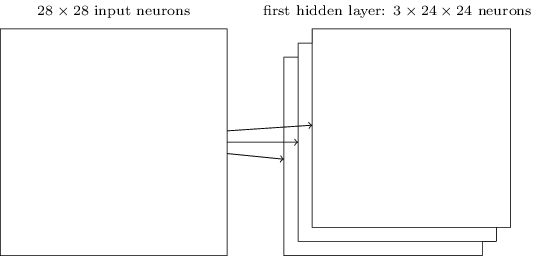
\includegraphics[scale=0.6]{res/cnn2.png}
\caption[Caption for LOF]{Warstwa wejściowa konwolucyjnej sieci neuronowej przedstawiona w trzech wymiarach. Źródło:\cite{nielsen}\label{cnn2}} 
\end{figure}

W sieciach konwolucyjnych, oprócz warstw konwolucyjnych, występują także warstwy typu \textit{pooling}, które pozwalają na pomniejszenie obrazu, co z kolei redukuje w pewnym stopniu koszty związane z obliczeniami. Jedną z podstawowych wykorzystywanych technik jest tzw. \textit{max-pooling}. Ponownie używając maski dowolnego rozmiaru (zazwyczaj $2x2$) ,,przechodzimy'' po całym obrazie, lecz tym razem wybierając do warstwy po operacji \textit{poolingu} piksel o najwyższej wartości.

\begin{figure}[ht!]
\centering
% obrazek pobrany z 
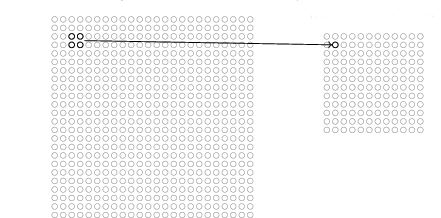
\includegraphics[scale=0.6]{res/pooling.png}
\caption[Caption for LOF]{Warstwa typu \textit{pooling}. Źródło:\cite{nielsen}\label{pooling}} 
\end{figure}

Po warstwach konwolucyjnych oraz typu \textit{pooling}, których ilość jest arbitralna, następuję przejście do tradycyjnych sieci neuronowych, gdzie dokonywana jest ostateczna klasyfikacja. Cała architektura przedstawiona została na rysunku \ref{cnn3}.

\begin{figure}[ht!]
\centering
% obrazek pobrany z https://www.kernix.com/blog/a-toy-convolutional-neural-network-for-image-classification-with-keras_p14
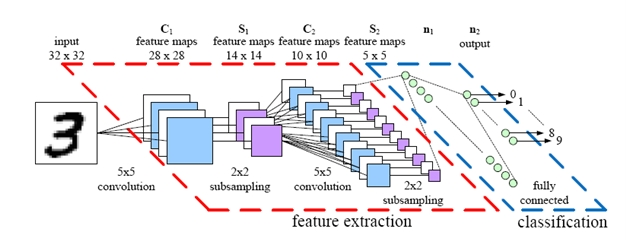
\includegraphics[scale=0.75]{res/cnn3.jpg}
\caption[Caption for LOF]{Architektura konwolucyjnych sieci neuronowych\footnotemark\label{cnn2}} 
\end{figure}
\footnotetext{\url{ https://www.kernix.com/blog/a-toy-convolutional-neural-network-for-image-classification-with-keras_p14}}

\subsection{Wykorzystane metody optymalizacji}
\subsubsection{Walidacja krzyzowa - wyznaczanie parametrow modelu}
\subsubsection{Sztuczne powiekszanie zbioru danych}
\subsubsection{Ekstrakcja cech}
\subsection{Problemy wynikające z niskiej ilości danych?}\label{problems}
\subsection{Proponowane rozwiązania?}
\paragraph{LDA}
\paragraph{PCA}

